\title{\bf Foundations2 \\Assignment 2020\\ Turing Machine multiplier\\}
\author{Sam Fay-Hunt \texttt{sf52@hw.ac.uk}}
\documentclass[11pt]{article} 
\usepackage{amsmath}
\usepackage{graphicx}

\graphicspath{ {./images/} }

\begin{document}
\date{}
\maketitle

\tableofcontents
\pagebreak

\section{Turing machine multiplication}
\subsection{Graph}
\begin{center}
  \makebox[\textwidth]{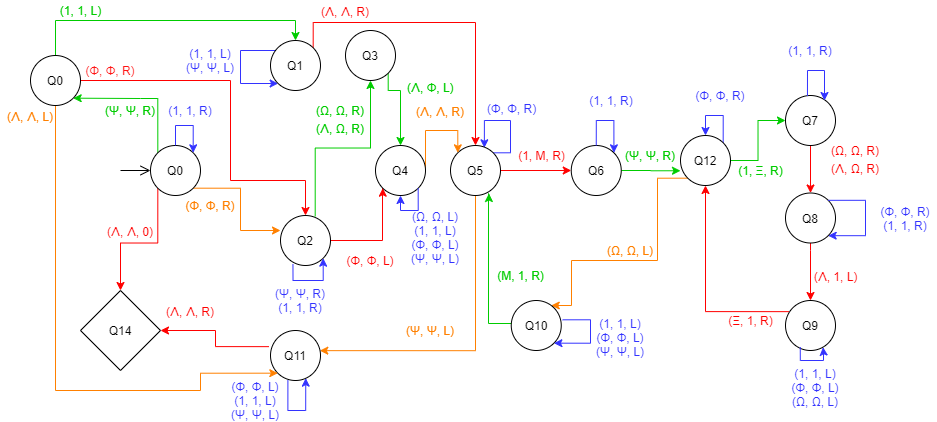
\includegraphics[width=0.9\paperwidth]{Turing-mult}}
\end{center}

\subsection{Formal definition}

$States = \{q_0, q_1, q_2, q_3, q_4, q_5, q_6, q_7, q_8, q_9, q_{10}, q_{11}, q_{12}\}$\\
$Symbols = \{\wedge, \Phi, \Psi, \Omega, 1, M, \Xi \}$
\begin{align*}
M_{ex}(q_0, \wedge) &= (q_{12}, \wedge, 0)    &     M_{ex}(q_0, 1) &= (q_{0}, 1, R) \\
M_{ex}(q_{0}, \Psi) &= (q_{1}, \Psi, R)    &     M_{ex}(q_{0}, \Phi) &= (q_{2}, \Phi, R) \\
M_{ex}(q_{1}, 1) &= (q_{1}, 1, L)    &     M_{ex}(q_{1}, \Psi) &= (q_{1}, \Psi, L) \\
M_{ex}(q_{1}, \wedge) &= (q_{5}, \wedge, R)    &     M_{ex}(q_{1}, \Phi) &= (q_{2}, \Phi, R) \\
M_{ex}(q_{2}, 1) &= (q_{2}, 1, R)    &     M_{ex}(q_{2}, \Psi) &= (q_{2}, \Psi, R) \\
M_{ex}(q_{2}, \wedge) &= (q_{3}, \Omega, R)    &     M_{ex}(q_{2}, \Omega) &= (q_{3}, \Omega, R) \\
M_{ex}(q_{2}, \Phi) &= (q_{4}, \Phi, L)    &     M_{ex}(q_{3}, \wedge) &= (q_{4}, \Phi, L) \\
M_{ex}(q_{4}, \Omega) &= (q_{4}, \Omega, L)    &     M_{ex}(q_{4}, 1) &= (q_{4}, 1, L) \\
M_{ex}(q_{4}, \Phi) &= (q_{4}, \Phi, L)    &     M_{ex}(q_{4}, \Psi) &= (q_{4}, \Psi, L) \\
M_{ex}(q_{4}, \wedge) &= (q_{5}, \wedge, R)    &     M_{ex}(q_{5}, \Phi) &= (q_{5}, \Phi, R) \\
M_{ex}(q_{5}, 1) &= (q_{6}, M, R)    &     M_{ex}(q_{5}, \Psi) &= (q_{11}, \Psi, L) \\
M_{ex}(q_{6}, \Phi) &= (q_{6}, \Phi, R)    &     M_{ex}(q_{6}, \Psi) &= (q_{6}, \Psi, R) \\
M_{ex}(q_{6}, 1) &= (q_{7}, \Xi, R)    &     M_{ex}(q_{6}, \Omega) &= (q_{10}, \Omega, L) \\
M_{ex}(q_{7}, \Omega) &= (q_{8}, \Omega, R)    &     M_{ex}(q_{7}, \wedge) &= (q_{8}, \Omega, R) \\
M_{ex}(q_{7}, 1) &= (q_{7}, 1, R)	&	M_{ex}(q_{8}, \wedge) &= (q_{9}, 1, L) \\
M_{ex}(q_{8}, 1) &= (q_{8}, 1, R)	&	M_{ex}(q_{8}, \Phi) &= (q_{8}, \Phi, R) \\
M_{ex}(q_{9}, 1) &= (q_{9}, 1, L)	&	M_{ex}(q_{9}, \Phi) &= (q_{9}, \Phi, L) \\
M_{ex}(q_{9}, \Omega) &= (q_{9}, \Omega, L)	&	M_{ex}(q_{9}, \Xi) &= (q_{6}, 1, R) \\
M_{ex}(q_{10}, 1) &= (q_{10}, 1, L)	&	M_{ex}(q_{10}, \Phi) &= (q_{10}, \Phi, L) \\
M_{ex}(q_{10}, \Psi) &= (q_{10}, \Psi, L)	&	M_{ex}(q_{10}, M) &= (q_{5}, 1, R) \\
M_{ex}(q_{11}, 1) &= (q_{11}, 1, L)	&	M_{ex}(q_{11}, \Phi) &= (q_{11}, \Phi, L) \\
M_{ex}(q_{11}, \wedge) &= (q_{12}, \wedge, R)	 \\
\end{align*}

\section{Discussion of graph}
\subsection{Logic of graph}
describe the logic of the graph, why I chose this logical method. consider the correctness.
\subsection{States \& Symbols}
Why I chose these states and symbols

cut down version here
\section{TM functionality}
How the graph works, where to start, where you end and dealing with 0, and negative numbers
\section{Implementation of Turing machine}
Language choice
\section{Tests}
Tests, inlcuding count of tapes printed, time to complete test
\section{Efficiency of program}
comment on the number of computation sequences produced and the time taked to complete each test
\section{Power of 3 machine}
asd
\end{document}